\documentclass{beamer}
\usepackage{listings}
\lstset{
%language=C,
frame=single, 
breaklines=true,
columns=fullflexible
}
\usepackage{subcaption}
\usepackage{url}
\usepackage{tikz}
\usepackage{graphicx}
\usepackage{tkz-euclide} % loads  TikZ and tkz-base
%\usetkzobj{all}
\usetikzlibrary{calc,math}
\usepackage{float}
\newcommand\norm[1]{\left\lVert#1\right\rVert}
\renewcommand{\vec}[1]{\mathbf{#1}}
\newcommand{\R}{\mathbb{R}}
\newcommand{\C}{\mathbb{C}}
\providecommand{\brak}[1]{\ensuremath{\left(#1\right)}}
\providecommand{\abs}[1]{\vert#1\vert}
\providecommand{\fourier}{\overset{\mathcal{F}}{ \rightleftharpoons}}
\providecommand{\pr}[1]{\ensuremath{\Pr\left(#1\right)}}
\providecommand{\sbrak}[1]{\ensuremath{{}\left[#1\right]}}
\usepackage[export]{adjustbox}
\usepackage[utf8]{inputenc}
\usepackage{amsmath}
\usetheme{Boadilla}
\title{Research Paper Presentation}
\author{Bokka Raja Ravi Kiran Reddy}
\date{CS20BTECH11009}
\begin{document}
%
\begin{frame}
\titlepage
\end{frame}
\begin{frame}
    \begin{block}{Title}
    A Bayesian Inference Approach for Location-Based Micro Motions using Radio Frequency Sensing
    \end{block}
    \begin{block}{Authors}
       David A. Maluf, Amr Elnakeeb, Matt Silverman
    \end{block}
    
\end{frame}
\begin{frame}
\begin{block}{Abstract}
\begin{enumerate}
    \item A Bayesian framework is proposed for the surface tracking objective\label{point-1}
    \item The resulting optimization problem, in which a non-linear forward model is linearized, is solved via gradient descent methods \label{point-2}
    \item  The location of the moving surface, the fractional area and the diffuse reflection coefficient as well as the velocity are inferred, versus time.\label{point-3}
    
\end{enumerate}
\end{block}
\end{frame}
\begin{frame}{Introduction}
\begin{enumerate}
    \item In the context of wireless localization ,Received Signal Strength Indication (RSSI) is used but it requires Line of sight (LOS) which is not guaranteed, especially in indoor environments. So, we use  Channel State Information (CSI) which suits for multipath environments and Non-Line of Sight (NLoS) communication—unlike RSSI.
    \item In the context of target tracking; herein, the proposed model is a parameterized signal strength model, from which synthetic observations are generated.
    \item For the case of wireless signals, we demonstrate how the moving micro surface areas, diffuse coefficients, locations and velocities can be inferred, based on the proposed model.
\end{enumerate}
\end{frame}


\begin{frame}{PROPOSED MODEL}
We assume that the transmitter is an isotropic source, and
the signal is reflected via the object surface then arrives at the receiving
radio end\\
We follow the free space attenuation model  that is, the received power at the
receiving antenna is given by,
\begin{align}
    P_{RX} = \frac{A_{RX}}{4\pi R^2} P_{TX}
\end{align}
where, R is the distance between that object (surface) and the receiving end.
 In terms of electric field strength ,
 \begin{align}
      P_{RX} = \frac{\lvert E_{r} \rvert ^2}{Z_{0}} A_{RX}\\
      P_{TX} = \frac{\lvert E_{s} \rvert ^2}{Z_{0}} \rho A_{e}
 \end{align}
 where,, $Z_0$ is the impedance of free space $\lvert E_{r} \rvert $ and $\lvert E_{s} \rvert $ are the magnitude of the electric field
strength at the receiving and transmitting ends, $\rho A_{e}$ effective surface area of the object.
 \end{frame}
 \begin{frame}{PROPOSED MODEL}
 By combining ,
 \begin{align}
     \lvert E_{r} \rvert = \frac{\sqrt{\rho A_{e}}}{2\sqrt{\pi} R} \lvert E_{s} \rvert
 \end{align}
 Define the normalized magnitude of electric field strengths as
M, 
\begin{align}
     M = \frac{\lvert E_{r} \rvert}{\lvert E_{s} \rvert} = \frac{\sqrt{\rho A_{e}}}{2\sqrt{\pi} R}
\end{align}
The phase difference between the received and
transmitted electric field is defined as,
\begin{align}
    \psi = \psi_{E_{r}} - \psi_{E_{s}} 
\end{align}
The measured phase is folded/wrapped due to the recurrence
characteristic of phase. Therefore, the measured phase has to
be transformed into the true “unwrapped” value.

    
\end{frame}
\begin{frame}{PROPOSED MODEL}
\begin{block}{Phase Unwrapping Algorithm}
\begin{enumerate}
    \item \boldsymbol{Input}:Measured (wrapped) phase $\psi_l$ of L
subcarriers; $l$ = 1, 2, . . . , L.
\item \boldsymbol{output} : Unwrapped phase $\phi_l$ of L subcarriers
\item \boldsymbol{Initialization} : Initialize $\psi_l=\phi_l$
, d = 0
\item for $l=2$ : L do\\
      If  $\psi_l-\psi_{l-1}> \pi$ then $d=d+1$\\
      $\phi_l=\psi_l-2\pi d$
      \item \boldsymbol{end for}
\end{enumerate}

\end{block}
Then, we write the
difference between the unwrapped phases as follows,
\begin{align}
     \phi = \phi_{E_{r}} - \phi_{E{s}} = -\frac{2\pi}{\lambda}(2R) = -\frac{4\pi}{\lambda}R
\end{align}
\end{frame}
\begin{frame}{PROPOSED MODEL}
\begin{figure}[h]
    \centering
    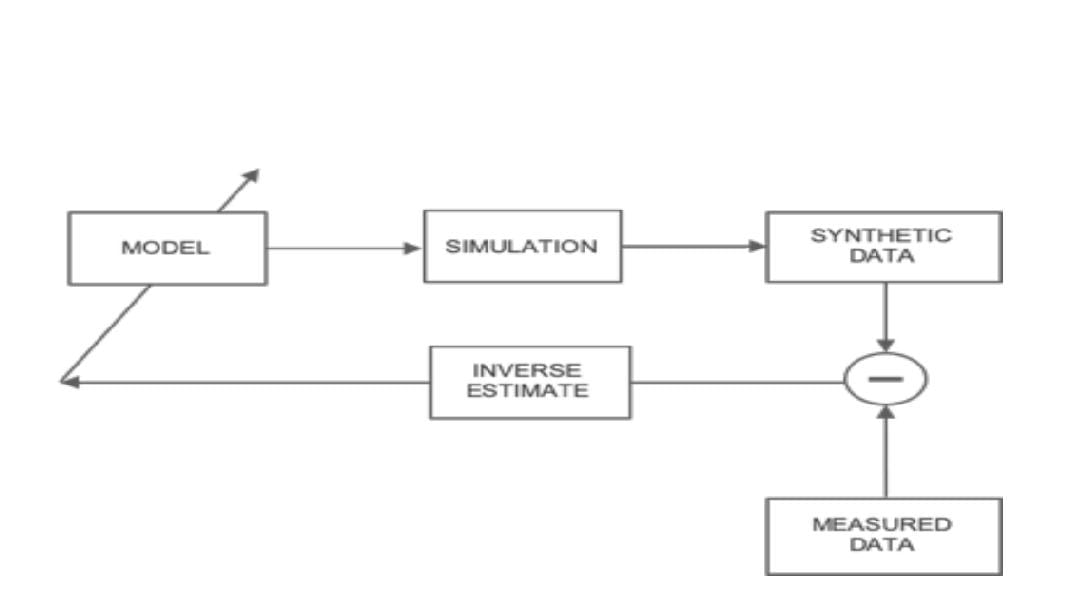
\includegraphics[width=6cm, height=4cm]{Figure.jpeg}
    \caption{Signal Model}
    \label{fig:Result4}
\end{figure}
 The error between
the real measurements and the synthetic observations is fed
to the simulator, through which the system parameters are
accordingly adjusted, to minimize the error in the subsequent
instances of time. Put differently, the estimation of the errors
means the system parameters are updated whenever more
measurements are available.

 
\end{frame}

\begin{frame}{BAYESIAN FRAMEWORK AND PROPOSED ALGORITHM}
    The object of interest has an effective surface area $\rho A_e$,
and is located at distance $R_i$ from the i-th access point,
i = 1, 2, . . . , N, where N denotes the total number of access
points. We assume that not all matter moves at once, and for
an infinitesimal period of time, motion is characterized by fractional effective surface $\rho A_e$ that has moved a distance $d\lambda$.\\
The full vector of distances and differential surface area is
defined as,
\begin{align}
    \boldsymbol{u}=[R_1,R_2,...,R_N,\bar{A_e}] \in \mathbb{R}^{N+1}
\end{align}
To estimate u from the collected measurements, we apply Bayes theorem,
\begin{align}
      \mathit{p}(\boldsymbol{u}|dM_1,....,dM_N) \propto \mathit{p}(dM_1,....,dM_N|\boldsymbol{u})\mathit{p}(\boldsymbol{u})
  \end{align} 
wherewhere, $dM_i$; i = 1, 2, . . . , N, is the differential component
of the magnitude of the signal strength on the i-th access
point. $\mathit{p}(\boldsymbol{u})$ is prior distribution of the
distances and surface area.\\
Furthermore, the prior distribution
is assumed to be zero-mean Gaussian, that is,
\end{frame}
\begin{frame}{BAYESIAN FRAMEWORK AND PROPOSED ALGORITHM}
\begin{align}
        p(\boldsymbol{u})\propto exp\brak{-\frac{1}{2}\boldsymbol{u}\boldsymbol{\Sigma^{-1}}\boldsymbol{u}^{\top}}
    \end{align}
    where,${\Sigma^{-1}} \in \mathbb{R}^{N+1\times N+1}$is the inverse covariance matrix
    \begin{align}
    \boldsymbol{\Sigma^{-1}}=\frac{4\pi}{\lambda}\begin{pmatrix}
\chi_1 & 0      & \cdots & 0       & 0 \\
0      & \chi_2 & \cdots & 0       & 0 \\
\vdots & \vdots & \ddots & \vdots  & \vdots  \\
0      & 0      & \cdots & \chi_{N}& 0\\
0      &0       &\cdots  &0        & 1
\end{pmatrix}
\end{align}
We penalize over the average difference, on each access point, between the
differential distances $dR_{ij}$ and the phase shifts $\frac{\lambda}{4\pi}d\phi_{ij}$ from angles of arrival.
\end{frame}
\begin{frame}{BAYESIAN FRAMEWORK AND PROPOSED ALGORITHM}
\begin{align}
        \chi_i = \frac{1}{\binom{V_i}{2}}\sum_{k,j,k\neq j}^{\binom{V_i}{2}}\brak{dR_{kj_i}-\frac{\lambda}{4\pi}d\phi_{kj_i}}^2
    \end{align}
    where k, j denote two antennas’ indices on any particular
access point i; i = 1, 2, . . . , N,. $V_i$ denotes the number
of antennas on the i-th access point.\\
We will take 2 Assssumptions.
\begin{enumerate}
    \item The difference between the measured real data and
the synthesized observed data follows a zero mean Gaussian
distribution 
\item The measurements are conditionally independent
\end{enumerate}
from this we get,
\end{frame}
\begin{frame}{BAYESIAN FRAMEWORK AND PROPOSED ALGORITHM}
 \begin{align}
       \mathit{p}(dM_1,....,dM_N|\boldsymbol{u})\propto exp\brak{-\frac{\sum_{i=1}^{N}\brak{dM_i-\hat{m}_i(\boldsymbol{u})}^2}{2\sigma^2}} 
    \end{align}
    where,$\hat{m}_i(\boldsymbol{u})$denotes estimated differential magnitude on
the i-th AP, and $\sigma^2$ is the noise variance.Therefore, the negative-log posterior is written as,
\begin{align}\label{negative-log posterior}
        \mathcal{L}(\boldsymbol{u})\propto -\frac{\sum_{i=1}^{N}\brak{dM_i-\hat{m}_i(\boldsymbol{u})}^2}{2\sigma^2} + \boldsymbol{u}\Sigma^{-1}\boldsymbol{u}^{\top} 
    \end{align}
\eqref{negative-log posterior} is a nonlinear function of u; and the MAP estimate is that value of u which minimizes $\mathcal{L}(\boldsymbol{u})$.
The vector of synthesized magnitudes of the motion is denoted by ,$\hat{m}(\boldsymbol{u})$, which is linearized about the current estimate, that is,
\begin{align}
        \hat{m}(\boldsymbol{u})=\hat{m}(\boldsymbol{u_0})+\boldsymbol{D}(\boldsymbol{u}-\boldsymbol{u_0})
    \end{align}
\end{frame}
\begin{frame}{BAYESIAN FRAMEWORK AND PROPOSED ALGORITHM}
D is written as,
    \begin{align}
        \boldsymbol{D} = \begin{pmatrix}
-\frac{\sqrt{\bar{A_e}}}{R_1^2} & \frac{\sqrt{\bar{A_e}}}{R_1R_2}      & \cdots & \frac{\sqrt{\bar{A_e}}}{R_1R_N}       & \frac{1}{2R_1\sqrt{\bar{A_e}}} \\
\frac{\sqrt{\bar{A_e}}}{R_2R_1}     & -\frac{\sqrt{\bar{A_e}}}{R_2^2} & \cdots & \frac{\sqrt{\bar{A_e}}}{R_2R_N}      & \frac{1}{2R_2\sqrt{\bar{A_e}}}\\
\vdots & \vdots & \ddots & \vdots  & \vdots  \\
 \frac{\sqrt{\bar{A_e}}}{R_NR_1}    & \frac{\sqrt{\bar{A_e}}}{R_NR_2}     & \cdots & -\frac{\sqrt{\bar{A_e}}}{R_N^2}&\frac{1}{2R_N\sqrt{\bar{A_e}}}  
\end{pmatrix}
    \end{align}
    The minimization of $\mathcal{L}(\boldsymbol{u})$ can be replaced with the
minimization of the following quadratic form\\
    \begin{align}
   \mathcal{L}^{\prime}&=\frac{1}{2}\boldsymbol{x}\boldsymbol{A}\boldsymbol{x}^{\top}-\boldsymbol{b}\boldsymbol{x}\\
   \boldsymbol{x}&= \boldsymbol{u}-\boldsymbol{u_0}\\
   \end{align}
\end{frame}
\begin{frame}{BAYESIAN FRAMEWORK AND PROPOSED ALGORITHM}
\begin{align}
\boldsymbol{A}&= \Sigma^{-1}-\frac{\boldsymbol{D}\boldsymbol{D}^{\top}}{\sigma^2}\\
   \boldsymbol{b}&=\boldsymbol{D}\frac{\brak{m(\boldsymbol{u})-\hat{m}(\boldsymbol{u})}}{\sigma^2}+\Sigma^{-1}\boldsymbol{u_0}
\end{align}

We search for the minimum in x in using a conjugate gradient method. At the minimum,we update the current estimate $u = u_0 + x$, recompute $\hat{m}(\boldsymbol{u})$ and D, and repeat the minimization procedure iteratively until the current estimate converges.\\

\end{frame}
\begin{frame}{BAYESIAN FRAMEWORK AND PROPOSED ALGORITHM}
Once again, using
Bayes theorem
\begin{align}
       \mathit{p}(x,y,z,s|\boldsymbol{u})\propto \mathit{p}(\boldsymbol{u}|x,y,z,s)\mathit{p}(x,y,z,s)
   \end{align} 
   where (x, y, z) is the position of the moving surface and s is a
scale.\\
The position of the moving surface and the scale are
estimated by solving the following set of N quadratic
equations.
\begin{align}
    (x-x_i)^2+(y-y_i)^2+(z-z_i)^2=sR_i^2,\hspace{0.5cm}
    i=1,...,N
    \end{align}
The method of choice is Levenberg–Marquardt minimization.\\
The corresponding velocities are estimated as follows,
 \begin{align}
        v_{x_i}^2+v_{y_i}^2+v_{z_i}^2= \brak{\frac{\frac{\lambda}{4\pi}d\phi_{t,t-1}}{dt}}_{i}^2,\hspace{0.5cm} i=1,...,N
    \end{align}
    where t is the time index

\end{frame}
\begin{frame}{Results}
   In our experiments, the CSI is collected from Cisco 4800 WiFi APs (Cisco Systems Inc., San Jose, CA, USA) on the 5 GHz radio frequency for WiFi. \\
   We use three APs for 2D inference. The three APs are placed to form a triangle, and they are put on desks
   \begin{figure}[h]
    \centering
    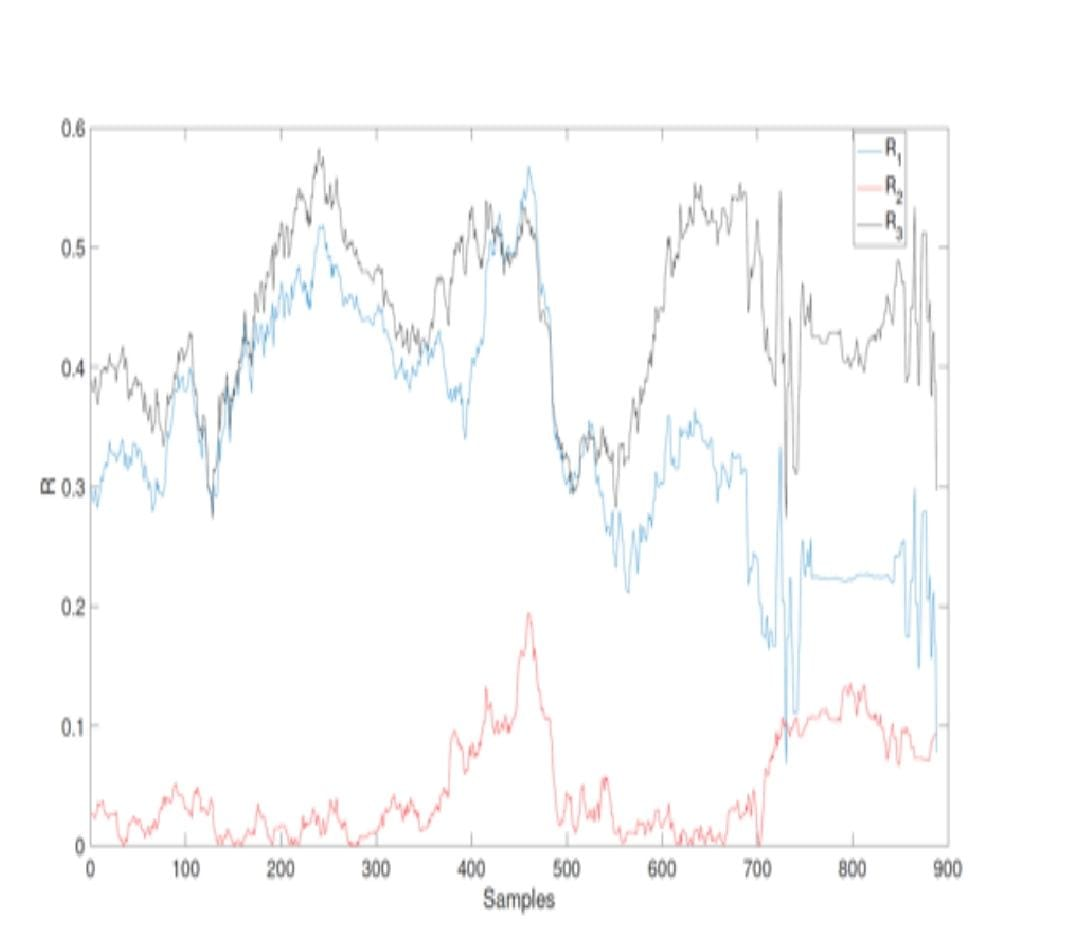
\includegraphics[width=6cm, height=4cm]{Result1.jpeg}
    \caption{Distances from the three APs in meters.}
    \label{fig:Result1}
\end{figure}
\end{frame}
\begin{frame}{Results}
\begin{figure}[h]
    \centering
    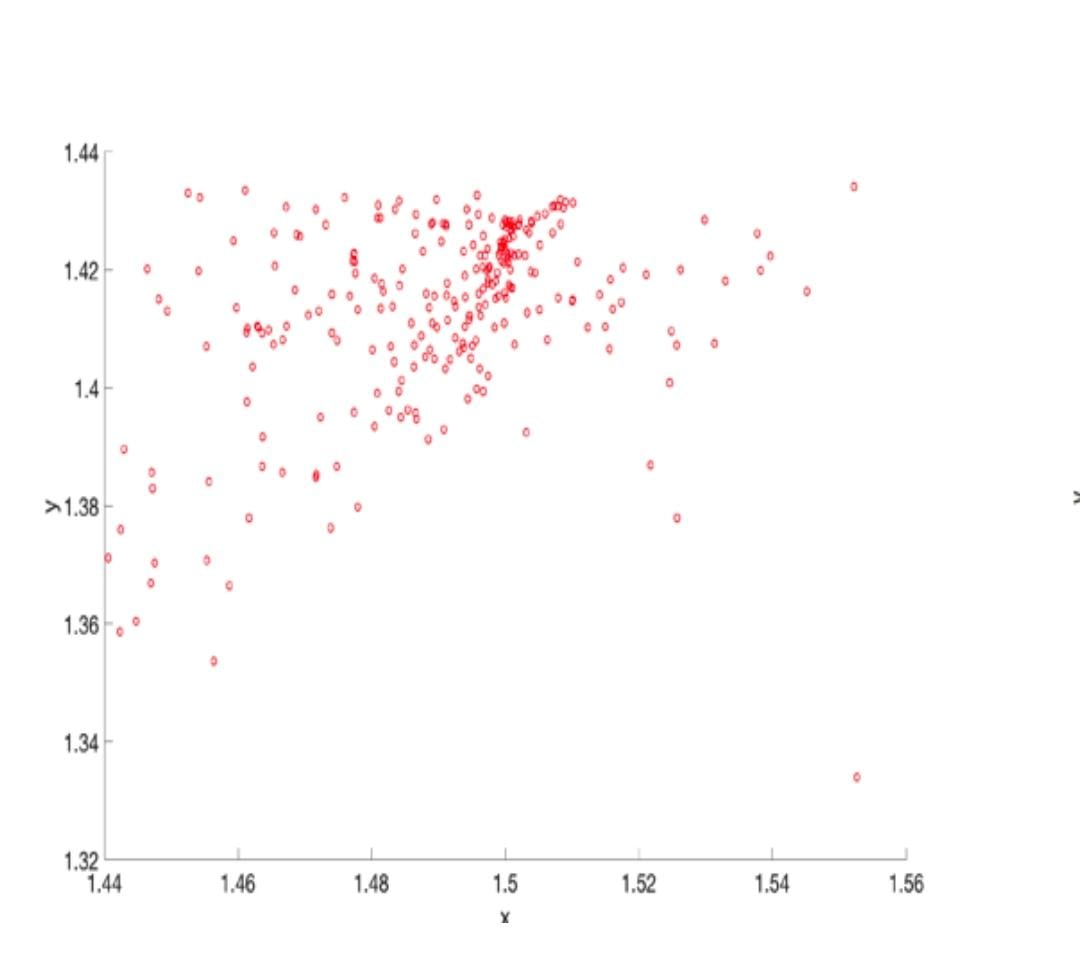
\includegraphics[width=5cm, height=3cm]{Result2.jpeg}
    \caption{(x, y) positions in meters}
    \label{fig:Result2}
\end{figure}
\begin{figure}[h]
    \centering
    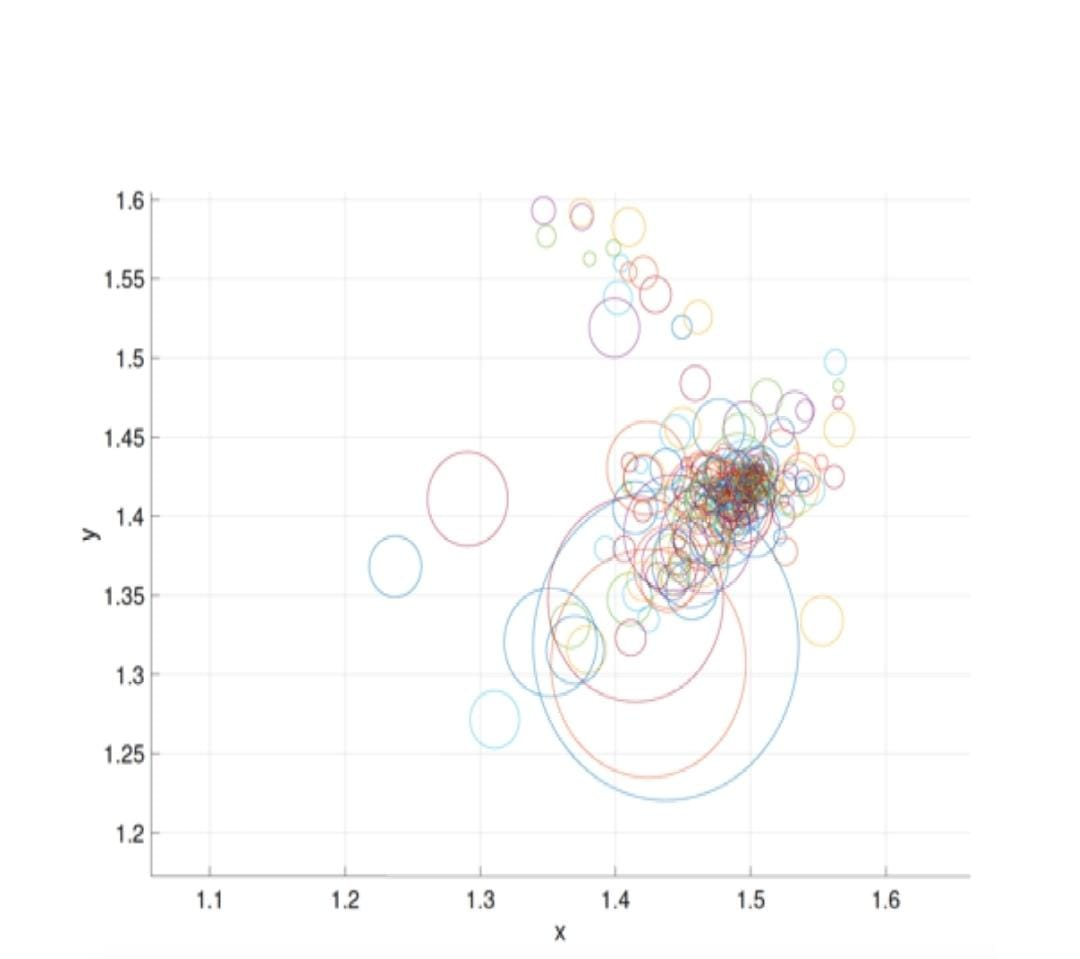
\includegraphics[width=5cm, height=3cm]{Result3.jpeg}
    \caption{Point spread function in meters}
    \label{fig:Result3}
\end{figure}
\end{frame}
\begin{frame}{Results}
\begin{figure}[h]
    \centering
    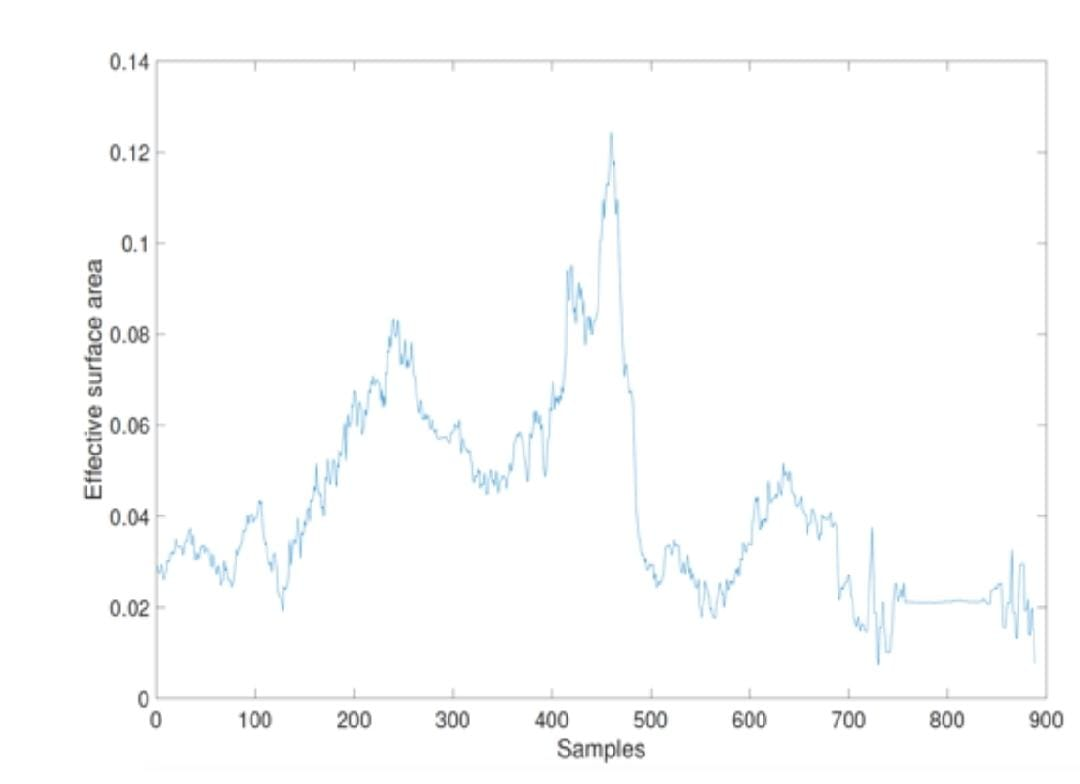
\includegraphics[width=6cm, height=4cm]{Result4.jpeg}
    \caption{. Effective surface area of the moving surface in $m^2$.}
    \label{fig:Result4}
\end{figure}
    
    
\end{frame}

\begin{frame}{Conclusion}
\begin{enumerate}
    \item A general inference framework has been proposed for the tracking of general moving micro surfaces,where the model choice is determined by the natural and physical properties of the surface we infer.
    
    \item Bayesian inferenceis formulated, and a combination of gradient descent and Levenberg–Marquardt algorithms is conducted.
\end{enumerate} 
\end{frame}

\end{document}
